% raw cheat sheet: two landscape A4 pages.  Build: make cheatsheet
% Every number here comes from lib/raw_ctl.h and lib/raw_voice.h
% (dial values printed from that code).
\documentclass{article}
\usepackage[a4paper,landscape,margin=6mm]{geometry}
\usepackage[T1]{fontenc}
\usepackage{lmodern}
\usepackage[default]{sourcesanspro}
\usepackage{amssymb}
\usepackage{amsmath}
\usepackage{tikz}
\usepackage[most]{tcolorbox}
\usepackage{array}
\usepackage{tabularx}
\pagestyle{empty}
\setlength{\parindent}{0pt}

\definecolor{ink}{RGB}{30,30,30}
\definecolor{snd}{RGB}{20,20,20}       % SOUND-page knob labels
\definecolor{modc}{RGB}{0,130,120}     % MOD-page knob labels
\definecolor{fxc}{RGB}{30,90,170}      % FX-page knob labels
\definecolor{vcoc}{RGB}{170,90,20}     % oscillators
\definecolor{fltc}{RGB}{190,40,60}     % filters
\definecolor{egc}{RGB}{150,60,170}     % envelopes
\definecolor{freec}{RGB}{170,170,170}  % unassigned
\definecolor{padc}{RGB}{120,170,230}

\newcommand{\MD}[1]{\textcolor{modc}{#1}}
\newcommand{\FX}[1]{\textcolor{fxc}{#1}}
\newcommand{\VC}[1]{\textcolor{vcoc}{#1}}
\newcommand{\FL}[1]{\textcolor{fltc}{#1}}
\newcommand{\EG}[1]{\textcolor{egc}{#1}}
\newcommand{\FR}[1]{\textcolor{freec}{#1}}
\newcommand{\cc}[1]{\textcolor{black!45}{\fontsize{4.6}{5}\selectfont #1}}

% knob: x, SOUND label (above), MOD and FX labels (below)
\newcommand{\knob}[4]{%
  \draw[fill=black!8, draw=black!60, line width=0.4pt] (#1,63) circle (3.4);
  \draw[black!60, line width=0.5pt] (#1,63) -- ++(110:2.9);
  \node[font=\fontsize{5.4}{6}\selectfont\bfseries, text=snd, align=center] at (#1,70.2) {#2};
  \node[font=\fontsize{5.2}{5.8}\selectfont, text=modc, align=center] at (#1,56.6) {#3};
  \node[font=\fontsize{5.2}{5.8}\selectfont, text=fxc, align=center] at (#1,52.4) {#4};}
\newcommand{\pad}[3]{%
  \draw[rounded corners=0.8mm, fill=padc!35!white, draw=padc!80!black, line width=0.4pt]
    (36+#1*13.2, 19+#2*13.2) rectangle ++(12,12);
  \node[font=\fontsize{5.4}{6}\selectfont, text=ink, align=center, text width=11mm]
    at (36+#1*13.2+6, 19+#2*13.2+6) {#3};}
\newcommand{\fader}[3]{%
  \draw[fill=black!12, draw=black!50] (#1-0.7,26) rectangle (#1+0.7,50);
  \draw[fill=#3!60!white, draw=#3!70!black, rounded corners=0.4mm] (#1-2.6,36) rectangle (#1+2.6,40);
  \node[font=\fontsize{5.4}{6}\selectfont\bfseries, text=#3!70!black, align=center] at (#1,55) {#2};}
\newcommand{\btn}[5]{%
  \draw[rounded corners=0.6mm, fill=#4!25!white, draw=#4!70!black, line width=0.4pt]
    (#1-#5/2,#2-2.6) rectangle (#1+#5/2,#2+2.6);
  \node[font=\fontsize{4.9}{5.4}\selectfont, text=ink, align=center] at (#1,#2) {#3};}

\tcbset{card/.style={enhanced, colback=white, colframe=black!70, boxrule=0.5pt, arc=1.5mm,
    left=1.6mm, right=1.6mm, top=1.1mm, bottom=1.1mm, toptitle=0.6mm, bottomtitle=0.6mm,
    fonttitle=\bfseries\fontsize{8.6}{10}\selectfont, coltitle=white, colbacktitle=black!75,
    fontupper=\fontsize{7.1}{8.5}\selectfont, before skip=0mm, after skip=1.8mm}}
\newtcolorbox{card}[1]{card, title={#1}}
\newcolumntype{L}{>{\raggedright\arraybackslash}X}

\begin{document}

{\fontsize{16}{18}\selectfont\bfseries raw}\hspace{3mm}%
{\fontsize{9.5}{11}\selectfont Axoloti Core + Launchkey 49 MK3 (standalone mode) \textperiodcentered{}
a monosynth after the Korg MS-20 \textperiodcentered{} \texttt{patches/raw/raw\_v1.axp}}\hfill
{\fontsize{7}{8}\selectfont\color{black!55} v1.0 \textperiodcentered{} 2026-11-13 \textperiodcentered{} page 1 of 2}

\vspace{1.5mm}
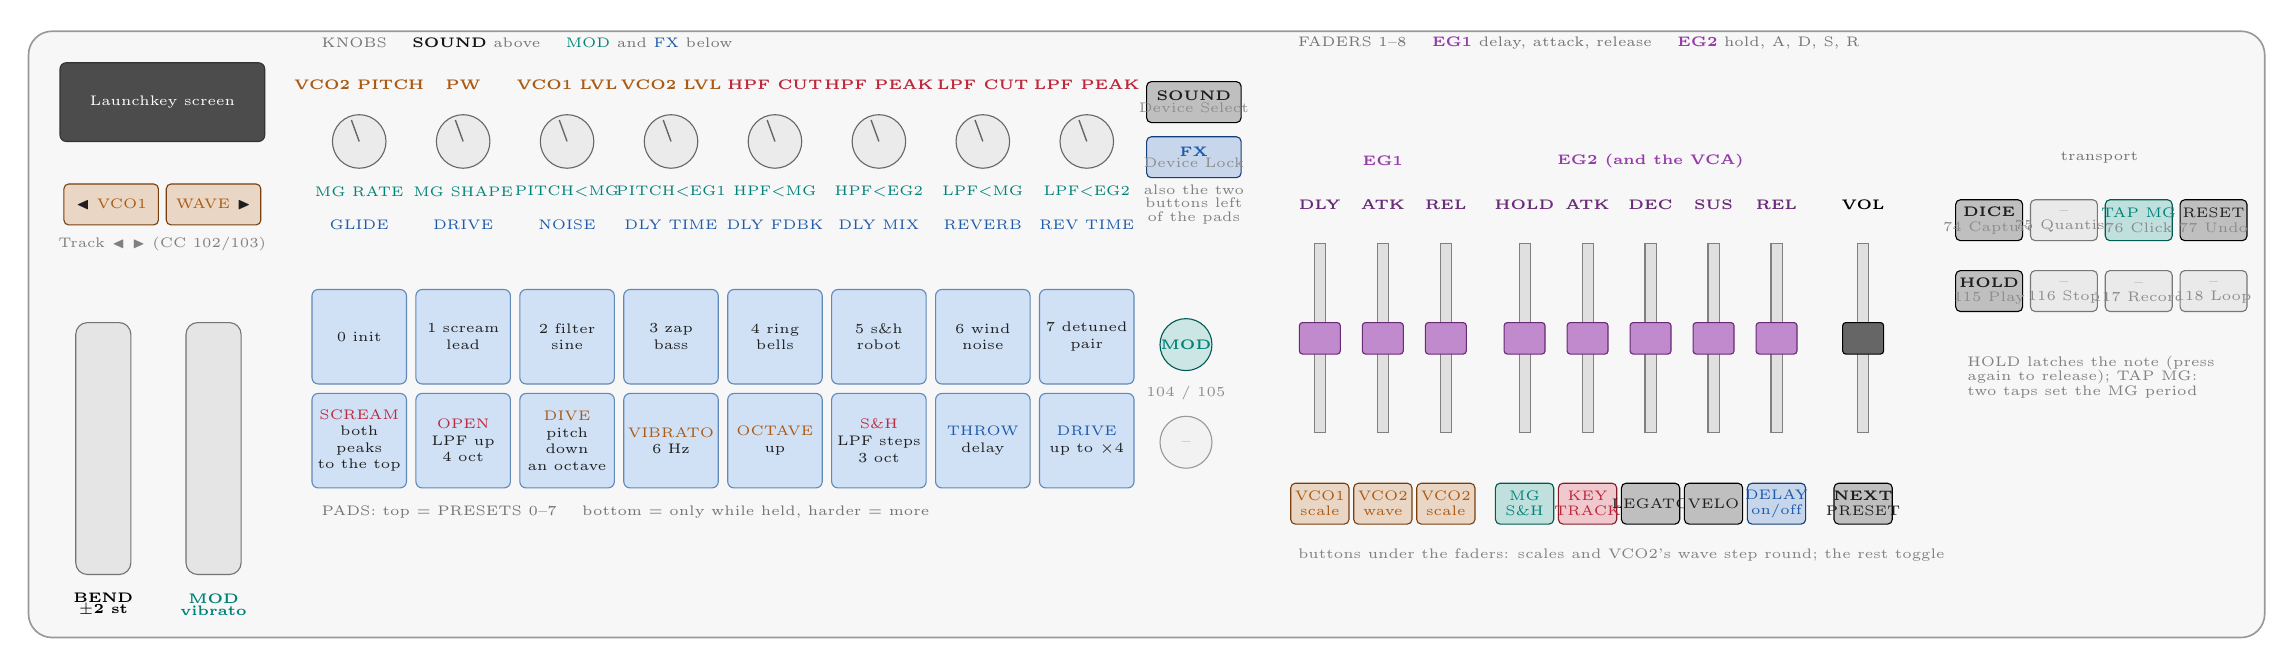
\begin{tikzpicture}[x=1mm,y=1mm]
  \draw[rounded corners=3mm, fill=black!3, draw=black!40, line width=0.6pt] (0,0) rectangle (284,77);

  % ---- left: screen, track buttons, wheels
  \draw[fill=black!70, draw=black!80, rounded corners=0.8mm] (4,63) rectangle (30,73);
  \node[font=\fontsize{5}{6}\selectfont, text=white] at (17,68) {Launchkey screen};
  \btn{10.5}{55}{\(\blacktriangleleft\) \VC{VCO1}}{vcoc}{12}
  \btn{23.5}{55}{\VC{WAVE} \(\blacktriangleright\)}{vcoc}{12}
  \node[font=\fontsize{4.6}{5}\selectfont, text=black!50] at (17,50) {Track \(\blacktriangleleft\) \(\blacktriangleright\) (CC 102/103)};
  \draw[rounded corners=1.5mm, fill=black!10, draw=black!55] (6,8) rectangle (13,40);
  \draw[rounded corners=1.5mm, fill=black!10, draw=black!55] (20,8) rectangle (27,40);
  \node[font=\fontsize{5.4}{6}\selectfont\bfseries, align=center] at (9.5,4.2) {BEND\\[-0.6mm]\(\pm\)2 st};
  \node[font=\fontsize{5.4}{6}\selectfont\bfseries, align=center, text=modc] at (23.5,4.2) {MOD\\[-0.6mm]vibrato};

  % ---- knobs: SOUND (top) / MOD (green) / FX (blue)
  \node[font=\fontsize{5}{6}\selectfont, text=black!55, anchor=west] at (36,75.5) {KNOBS \quad
     \textbf{\textcolor{snd}{SOUND}} above \quad \MD{MOD} and \FX{FX} below};
  \knob{42}{\VC{VCO2 PITCH}}{\MD{MG RATE}}{\FX{GLIDE}}
  \knob{55.2}{\VC{PW}}{\MD{MG SHAPE}}{\FX{DRIVE}}
  \knob{68.4}{\VC{VCO1 LVL}}{\MD{PITCH<MG}}{\FX{NOISE}}
  \knob{81.6}{\VC{VCO2 LVL}}{\MD{PITCH<EG1}}{\FX{DLY TIME}}
  \knob{94.8}{\FL{HPF CUT}}{\MD{HPF<MG}}{\FX{DLY FDBK}}
  \knob{108}{\FL{HPF PEAK}}{\MD{HPF<EG2}}{\FX{DLY MIX}}
  \knob{121.2}{\FL{LPF CUT}}{\MD{LPF<MG}}{\FX{REVERB}}
  \knob{134.4}{\FL{LPF PEAK}}{\MD{LPF<EG2}}{\FX{REV TIME}}
  \btn{148}{68}{\textbf{SOUND}\\[-0.4mm]\cc{Device Select}}{black}{12}
  \btn{148}{61}{\textbf{\FX{FX}}\\[-0.4mm]\cc{Device Lock}}{fxc}{12}
  \node[font=\fontsize{4.4}{5}\selectfont, text=black!50, align=center] at (148,55) {also the two\\buttons left\\of the pads};

  % ---- pads
  \pad{0}{1}{0 init} \pad{1}{1}{1 scream\\lead} \pad{2}{1}{2 filter\\sine} \pad{3}{1}{3 zap\\bass}
  \pad{4}{1}{4 ring\\bells} \pad{5}{1}{5 s\&h\\robot} \pad{6}{1}{6 wind\\noise} \pad{7}{1}{7 detuned\\pair}
  \pad{0}{0}{\FL{SCREAM}\\both peaks\\to the top} \pad{1}{0}{\FL{OPEN}\\LPF up\\4 oct} \pad{2}{0}{\VC{DIVE}\\pitch down\\an octave}
  \pad{3}{0}{\VC{VIBRATO}\\6 Hz} \pad{4}{0}{\VC{OCTAVE}\\up} \pad{5}{0}{\FL{S\&H}\\LPF steps\\3 oct}
  \pad{6}{0}{\FX{THROW}\\delay} \pad{7}{0}{\FX{DRIVE}\\up to \(\times\)4}
  \node[font=\fontsize{5}{6}\selectfont, text=black!55, anchor=west] at (36,16) {PADS: top = PRESETS 0--7 \quad bottom = only while held, harder = more};
  \draw[fill=modc!20, draw=modc!70!black] (147,37.2) circle (3.3);
  \draw[fill=black!5, draw=black!40] (147,24.8) circle (3.3);
  \node[font=\fontsize{4.6}{5}\selectfont\bfseries, text=modc] at (147,37.2) {MOD};
  \node[font=\fontsize{4.6}{5}\selectfont, text=freec] at (147,24.8) {--};
  \node[font=\fontsize{4.2}{5}\selectfont, text=black!45] at (147,31) {104 / 105};

  % ---- faders: EG1, EG2
  \node[font=\fontsize{5}{6}\selectfont, text=black!55, anchor=west] at (160,75.5) {FADERS 1--8 \quad
     \EG{\textbf{EG1}} delay, attack, release \quad \EG{\textbf{EG2}} hold, A, D, S, R};
  \fader{164}{DLY}{egc} \fader{172}{ATK}{egc} \fader{180}{REL}{egc}
  \node[font=\fontsize{5}{6}\selectfont\bfseries, text=egc] at (172,60.5) {EG1};
  \fader{190}{HOLD}{egc} \fader{198}{ATK}{egc} \fader{206}{DEC}{egc} \fader{214}{SUS}{egc} \fader{222}{REL}{egc}
  \node[font=\fontsize{5}{6}\selectfont\bfseries, text=egc] at (206,60.5) {EG2 (and the VCA)};
  \fader{233}{VOL}{black}
  \btn{164}{17}{\VC{VCO1}\\\VC{scale}}{vcoc}{7.4}
  \btn{172}{17}{\VC{VCO2}\\\VC{wave}}{vcoc}{7.4}
  \btn{180}{17}{\VC{VCO2}\\\VC{scale}}{vcoc}{7.4}
  \btn{190}{17}{\MD{MG}\\\MD{S\&H}}{modc}{7.4}
  \btn{198}{17}{\FL{KEY}\\\FL{TRACK}}{fltc}{7.4}
  \btn{206}{17}{LEGATO}{black}{7.4}
  \btn{214}{17}{VELO}{black}{7.4}
  \btn{222}{17}{\FX{DELAY}\\\FX{on/off}}{fxc}{7.4}
  \btn{233}{17}{\textbf{NEXT}\\PRESET}{black}{7.4}
  \node[font=\fontsize{4.6}{5}\selectfont, text=black!50, anchor=west] at (160,10.5) {buttons under the faders: scales and VCO2's wave step round; the rest toggle};

  % ---- transport (ch 16)
  \node[font=\fontsize{5}{6}\selectfont, text=black!55] at (263,61) {transport};
  \btn{249}{53}{\textbf{DICE}\\\cc{74 Capture}}{black}{8.5}
  \btn{258.5}{53}{\FR{--}\\\cc{75 Quantise}}{freec}{8.5}
  \btn{268}{53}{\MD{TAP MG}\\\cc{76 Click}}{modc}{8.5}
  \btn{277.5}{53}{RESET\\\cc{77 Undo}}{black}{8.5}
  \btn{249}{44}{\textbf{HOLD}\\\cc{115 Play}}{black}{8.5}
  \btn{258.5}{44}{\FR{--}\\\cc{116 Stop}}{freec}{8.5}
  \btn{268}{44}{\FR{--}\\\cc{117 Record}}{freec}{8.5}
  \btn{277.5}{44}{\FR{--}\\\cc{118 Loop}}{freec}{8.5}
  \node[font=\fontsize{4.6}{5.2}\selectfont, text=black!50, align=left, anchor=north west] at (245,37)
     {HOLD latches the note (press\\again to release); TAP MG:\\two taps set the MG period};
\end{tikzpicture}

\vspace{1.2mm}
\begin{minipage}[t]{72mm}\vspace{0pt}
\begin{card}{Signal path (as on the MS-20's panel)}
\VC{VCO1} (triangle, saw, pulse, noise) + \VC{VCO2} (saw, square, narrow pulse, ring) + noise \(\to\)
DRIVE \(\to\) \FL{HPF} \(\to\) \FL{LPF} \(\to\) VCA (\EG{EG2}) \(\to\) delay \(\to\) reverb \(\to\) VOL.
\MD{MG} (ramp down -- triangle -- ramp up, or S\&H), \EG{EG1} and \EG{EG2} modulate pitch and the two cutoffs.
\textbf{Mono}: the last key sounds; releasing it returns to the key still held.
\end{card}
\begin{card}{The filters}
Both are 2-pole (12 dB/oct) with clipping in the feedback loop, as the MS-20's Korg-35. PEAK
past \textbf{91\,\%} (knob 116): the filter \textbf{self-oscillates}, a sine at the cutoff that the
clipping keeps in bounds; louder input pushes against it (the scream). HPF then LPF: two peaks
make a band-pass with two resonances. \FL{KEY TRACK}: both cutoffs follow the keys an octave per
octave, so a self-oscillating filter plays in tune.
\end{card}
\end{minipage}\hfill
\begin{minipage}[t]{70mm}\vspace{0pt}
\begin{card}{Oscillators (fader buttons 1--3, Track)}
\fontsize{6.8}{8.1}\selectfont
\begin{tabularx}{\linewidth}{@{}l L@{}}
\VC{\textbf{VCO1 wave}} & Track \(\blacktriangleleft\blacktriangleright\): triangle, saw, pulse (width: PW), noise \\
\VC{\textbf{VCO1 scale}} & 32', 16', 8', 4' (8' = the key's pitch) \\
\VC{\textbf{VCO2 wave}} & saw, square, narrow pulse (15\,\%), ring (VCO1's square \(\times\) VCO2's square) \\
\VC{\textbf{VCO2 scale}} & 16', 8', 4', 2' \\
\VC{\textbf{VCO2 PITCH}} & \(\pm\)12 st, fine near the centre (centre = in tune) \\
\end{tabularx}
\end{card}
\begin{card}{Envelopes}
\EG{EG1}: after DELAY, rises in ATTACK, stays up while the key is held, falls in RELEASE.
PITCH<EG1: the pitch starts that far off (right of centre: above, a zap; left: below, a scoop) and
reaches the note as EG1 rises, so held notes stay in tune (the MS-20 adds EG1 to the pitch instead). \EG{EG2}: attack, decay, sustain, release; HOLD
keeps it going that long after the key is up. It drives the VCA and the filters' EG2 amounts.
\textbf{LEGATO}: keys played over a held key do not restart the envelopes.
\end{card}
\end{minipage}\hfill
\begin{minipage}[t]{66mm}\vspace{0pt}
\begin{card}{Pads}
\textbf{Top} = presets 0--7. \textbf{Bottom}, while held; strike velocity, then pressure, sets the amount:
\fontsize{6.6}{7.9}\selectfont
\begin{tabularx}{\linewidth}{@{}l L@{}}
\FL{SCREAM} & both PEAKs towards the top \\
\FL{OPEN} & LPF cutoff up to 4 octaves \\
\VC{DIVE} & pitch down, up to an octave \\
\VC{VIBRATO / OCTAVE} & 6 Hz \(\pm\)0.7 st / an octave up \\
\FL{S\&H} & random LPF steps at the MG rate, up to 3 oct \\
\FX{THROW} & delay throw (echoes ring on) \\
\FX{DRIVE} & drive up to \(\times\)4 \\
\end{tabularx}
\end{card}
\begin{card}{Wheels and transport}
MOD wheel: vibrato from the MG, up to 1 st (on top of PITCH<MG). Bend \(\pm\)2 st.
DICE rolls waves, scales and the SOUND and MOD pages (envelopes, FX, volume stay). RESET = preset 0.
\end{card}
\end{minipage}\hfill
\begin{minipage}[t]{68mm}\vspace{0pt}
\begin{card}{Inside}
\fontsize{6.6}{7.8}\selectfont
Filters: Sallen--Key 2-pole, \(H_{LP} = \omega^2/(s^2 + (2-k)\omega s + \omega^2)\), zero-delay feedback
(trapezoidal), a cubic clip in the feedback; each sample solves one scalar equation, which has
exactly one root, by 2 Newton steps (measured error \(< 6\cdot10^{-5}\)). Self-oscillation from \(k = 2\).
The voice runs at 96 kHz (band-limited oscillators, drive and filters) and a half-band filter
(\(-79\) dB) brings it to 48 kHz. Envelopes per sample; pitch and cutoffs at 12 kHz.
Code: \texttt{lib/raw\_voice.h}.
\end{card}
\begin{card}{Load}
DSP 70.5--79.5\,\% (constant: the voice costs the same with or without a note; most for the ring), patch RAM 22 of 44 KB.
\end{card}
\end{minipage}

%======================================================================
\newpage
{\fontsize{16}{18}\selectfont\bfseries raw}\hspace{3mm}%
{\fontsize{9.5}{11}\selectfont presets, dial values, recipes, troubleshooting}\hfill
{\fontsize{7}{8}\selectfont\color{black!55} v1.0 \textperiodcentered{} page 2 of 2}

\vspace{1.5mm}
\begin{minipage}[t]{150mm}\vspace{0pt}
\begin{card}{Presets: top pads = 0--7; NEXT PRESET (fader button 9) steps; RESET (Undo) = 0 \quad\textmd{\fontsize{6.5}{7}\selectfont (chosen from the parameter meanings, not yet tuned by ear)}}
\fontsize{7.2}{8.7}\selectfont
\begin{tabularx}{\linewidth}{@{}>{\bfseries}l L@{}}
0 init & One saw through the LPF (peak 0.55 of the way), EG2 opens it 3.8 octaves. The power-on sound. \\
1 scream lead & Pulse + saw a little detuned, HPF at 180 Hz, LPF peak just below self-oscillation, drive, legato, glide, delay. \\
2 filter sine & The LPF self-oscillates and tracks the keys (KEY TRACK): a sine played by the filter (about 10 cents flat; LPF CUT steps are coarse), a little triangle and noise to start it. \\
3 zap bass & Saw + square at 16'; each note starts 13 st above and falls to pitch in 40 ms (EG1); short EG2 into a resonant LPF; velocity. \\
4 ring bells & VCO2 on ring, a fifth up, short-decay EG2, delay. \\
5 s\&h robot & MG on S\&H at 6.5 Hz steps the LPF 2.5 octaves around a resonant cutoff. \\
6 wind noise & VCO1 on noise; both filters resonant and slowly swept by the MG; slow EG2. \\
7 detuned pair & Pulse at 8' + saw at 4', 11 cents apart, EG2 into the LPF. \\
\end{tabularx}\\[0.3mm]
A preset sets the waves, scales, toggles, the three knob pages and the eight envelope faders; the volume stays.
\end{card}

\begin{card}{Recipes}
\fontsize{7.4}{9.0}\selectfont
\textbf{Scream}: LPF PEAK past 91\,\%, sweep LPF CUT, then add DRIVE or VCO levels: the input fights the
resonance.\quad
\textbf{Two peaks}: HPF and LPF PEAK both at 3/4, cutoffs a few octaves apart: a hollow, talking band.\quad
\textbf{Zap}: PITCH<EG1 right of centre, EG1 ATTACK at 1/3 (20 ms), legato off.\quad
\textbf{Filter as oscillator}: VCO levels down, LPF PEAK full, KEY TRACK on; tune with LPF CUT.\quad
\textbf{Sample and hold}: MG S\&H on, LPF<MG up, MG RATE to taste (or TAP MG).
\end{card}
\end{minipage}\hfill
\begin{minipage}[t]{128mm}\vspace{0pt}
\begin{card}{Where the values fall (knob turned \dots)}
\fontsize{7.5}{9.2}\selectfont
\setlength{\tabcolsep}{3pt}
\begin{tabular}{@{}l r r r r r@{}}
 & 0 & 1/4 & 1/2 & 3/4 & full \\ \hline
\FL{\textbf{HPF / LPF CUT}} (Hz) & 20 & 115 & 660 & 3600 & 20000 \\
\FL{\textbf{PEAK}} (Q) & 0.5 & 0.7 & 1.1 & 2.8 & self-osc. \\
\VC{\textbf{VCO2 PITCH}} (st) & \(-12\) & \(-3.1\) & 0 & \(+2.9\) & \(+12\) \\
\VC{\textbf{PW}} & 50\,\% & 39\,\% & 27\,\% & 16\,\% & 5\,\% \\
\MD{\textbf{MG RATE}} (Hz) & 0.1 & 0.48 & 2.3 & 11 & 51 \\
\MD{\textbf{MG SHAPE}} & ramp down & & triangle & & ramp up \\
\MD{\textbf{PITCH<MG}} (st) & 0 & 0.76 & 3 & 6.7 & 12 \\
\MD{\textbf{PITCH<EG1}} (st, start) & \(-24\) & \(-6.2\) & 0 & \(+5.8\) & \(+24\) \\
\MD{\textbf{HPF/LPF<MG}} (oct) & 0 & 0.3 & 1.3 & 2.8 & 5 \\
\MD{\textbf{HPF<EG2 / LPF<EG2}} (oct) & 0 & 1.5 / 2 & 3 / 4 & 4.5 / 6 & 6 / 8 \\
\FX{\textbf{GLIDE}} (s) & 0 & 0.13 & 0.5 & 1.1 & 2 \\
\FX{\textbf{DRIVE}} (gain) & 0.5 & 1 & 2 & 4 & 8 \\
\EG{\textbf{attack, decay, release}} (s) & 0.001 & 0.01 & 0.1 & 1 & 10 \\
\EG{\textbf{EG1 DELAY, EG2 HOLD}} (s) & 0 & 0.13 & 0.5 & 1.1 & 2 \\
\end{tabular}
\end{card}

\begin{card}{Something seems wrong?}
\fontsize{7.5}{9.2}\selectfont
\textbf{Silence}: VCO levels and NOISE at 0, LPF CUT at the bottom (or HPF CUT at the top), EG2 SUSTAIN 0 with a
short decay, or VOL down.\quad
\textbf{A note that will not stop}: HOLD is latched (Play).\quad
\textbf{Out of tune}: VCO2 PITCH off centre, or PITCH<EG1 off centre with a long EG1 ATTACK or DELAY (the note arrives late).\quad
\textbf{Lost}: RESET (Undo).\quad
\textbf{Another patch} (on the SD card): hold both buttons left of the pads and tap a top pad: 1 freak, 2 grains, 3 groove, 4 soliton, 5 aeolian, 6 raw, 7 quartet.
\end{card}
\end{minipage}

\end{document}
